%%%%%%%%%%%%%%%%%%%%%%%%%%%%%%%%%%%%%%%%%
% Lachaise Assignment
% LaTeX Template
% Version 1.0 (26/6/2018)
%
% This template originates from:
% http://www.LaTeXTemplates.com
%
% Authors:
% Marion Lachaise & François Févotte
% Vel (vel@LaTeXTemplates.com)
%
% License:
% CC BY-NC-SA 3.0 (http://creativecommons.org/licenses/by-nc-sa/3.0/)
% 
%%%%%%%%%%%%%%%%%%%%%%%%%%%%%%%%%%%%%%%%%

%----------------------------------------------------------------------------------------
%	PACKAGES AND OTHER DOCUMENT CONFIGURATIONS
%----------------------------------------------------------------------------------------

\documentclass{article}
\usepackage{amsthm}
\usepackage{listings}
\usepackage{xcolor}
\usepackage{graphicx}


\lstset{
	language=Python,
	basicstyle=\ttfamily\small,
	keywordstyle=\color{blue},
	stringstyle=\color{red},
	commentstyle=\color{purple},
	showstringspaces=false,
	numbers=left,
	numberstyle=\tiny\color{gray},
	breaklines=true,
	frame=single,
	captionpos=b
}
\newtheorem{definition}{Definition}[section]
\newtheorem{proposition}{Proposition}
\newtheorem{corolary}{Corolary}

%%%%%%%%%%%%%%%%%%%%%%%%%%%%%%%%%%%%%%%%%
% Lachaise Assignment
% Structure Specification File
% Version 1.0 (26/6/2018)
%
% This template originates from:
% http://www.LaTeXTemplates.com
%
% Authors:
% Marion Lachaise & François Févotte
% Vel (vel@LaTeXTemplates.com)
%
% License:
% CC BY-NC-SA 3.0 (http://creativecommons.org/licenses/by-nc-sa/3.0/)
% 
%%%%%%%%%%%%%%%%%%%%%%%%%%%%%%%%%%%%%%%%%

%----------------------------------------------------------------------------------------
%	PACKAGES AND OTHER DOCUMENT CONFIGURATIONS
%----------------------------------------------------------------------------------------

\usepackage{amsmath,amsfonts,stmaryrd,amssymb} % Math packages

\usepackage{enumerate} % Custom item numbers for enumerations

\usepackage[ruled]{algorithm2e} % Algorithms

\usepackage[framemethod=tikz]{mdframed} % Allows defining custom boxed/framed environments

\usepackage{listings} % File listings, with syntax highlighting
\lstset{
	basicstyle=\ttfamily, % Typeset listings in monospace font
}

%----------------------------------------------------------------------------------------
%	DOCUMENT MARGINS
%----------------------------------------------------------------------------------------

\usepackage{geometry} % Required for adjusting page dimensions and margins

\geometry{
	paper=a4paper, % Paper size, change to letterpaper for US letter size
	top=2.5cm, % Top margin
	bottom=3cm, % Bottom margin
	left=2.5cm, % Left margin
	right=2.5cm, % Right margin
	headheight=14pt, % Header height
	footskip=1.5cm, % Space from the bottom margin to the baseline of the footer
	headsep=1.2cm, % Space from the top margin to the baseline of the header
	%showframe, % Uncomment to show how the type block is set on the page
}

%----------------------------------------------------------------------------------------
%	FONTS
%----------------------------------------------------------------------------------------

\usepackage[utf8]{inputenc} % Required for inputting international characters
\usepackage[T1]{fontenc} % Output font encoding for international characters

\usepackage{XCharter} % Use the XCharter fonts

%----------------------------------------------------------------------------------------
%	COMMAND LINE ENVIRONMENT
%----------------------------------------------------------------------------------------

% Usage:
% \begin{commandline}
%	\begin{verbatim}
%		$ ls
%		
%		Applications	Desktop	...
%	\end{verbatim}
% \end{commandline}

\mdfdefinestyle{commandline}{
	leftmargin=10pt,
	rightmargin=10pt,
	innerleftmargin=15pt,
	middlelinecolor=black!50!white,
	middlelinewidth=2pt,
	frametitlerule=false,
	backgroundcolor=black!5!white,
	frametitle={Command Line},
	frametitlefont={\normalfont\sffamily\color{white}\hspace{-1em}},
	frametitlebackgroundcolor=black!50!white,
	nobreak,
}

% Define a custom environment for command-line snapshots
\newenvironment{commandline}{
	\medskip
	\begin{mdframed}[style=commandline]
}{
	\end{mdframed}
	\medskip
}

%----------------------------------------------------------------------------------------
%	FILE CONTENTS ENVIRONMENT
%----------------------------------------------------------------------------------------

% Usage:
% \begin{file}[optional filename, defaults to "File"]
%	File contents, for example, with a listings environment
% \end{file}

\mdfdefinestyle{file}{
	innertopmargin=1.6\baselineskip,
	innerbottommargin=0.8\baselineskip,
	topline=false, bottomline=false,
	leftline=false, rightline=false,
	leftmargin=2cm,
	rightmargin=2cm,
	singleextra={%
		\draw[fill=black!10!white](P)++(0,-1.2em)rectangle(P-|O);
		\node[anchor=north west]
		at(P-|O){\ttfamily\mdfilename};
		%
		\def\l{3em}
		\draw(O-|P)++(-\l,0)--++(\l,\l)--(P)--(P-|O)--(O)--cycle;
		\draw(O-|P)++(-\l,0)--++(0,\l)--++(\l,0);
	},
	nobreak,
}

% Define a custom environment for file contents
\newenvironment{file}[1][File]{ % Set the default filename to "File"
	\medskip
	\newcommand{\mdfilename}{#1}
	\begin{mdframed}[style=file]
}{
	\end{mdframed}
	\medskip
}

%----------------------------------------------------------------------------------------
%	NUMBERED QUESTIONS ENVIRONMENT
%----------------------------------------------------------------------------------------

% Usage:
% \begin{question}[optional title]
%	Question contents
% \end{question}

\mdfdefinestyle{question}{
	innertopmargin=1.2\baselineskip,
	innerbottommargin=0.8\baselineskip,
	roundcorner=5pt,
	nobreak,
	singleextra={%
		\draw(P-|O)node[xshift=1em,anchor=west,fill=white,draw,rounded corners=5pt]{%
		Question \theQuestion\questionTitle};
	},
}

\newcounter{Question} % Stores the current question number that gets iterated with each new question

% Define a custom environment for numbered questions
\newenvironment{question}[1][\unskip]{
	\bigskip
	\stepcounter{Question}
	\newcommand{\questionTitle}{~#1}
	\begin{mdframed}[style=question]
}{
	\end{mdframed}
	\medskip
}

%----------------------------------------------------------------------------------------
%	WARNING TEXT ENVIRONMENT
%----------------------------------------------------------------------------------------

% Usage:
% \begin{warn}[optional title, defaults to "Warning:"]
%	Contents
% \end{warn}

\mdfdefinestyle{warning}{
	topline=false, bottomline=false,
	leftline=false, rightline=false,
	nobreak,
	singleextra={%
		\draw(P-|O)++(-0.5em,0)node(tmp1){};
		\draw(P-|O)++(0.5em,0)node(tmp2){};
		\fill[black,rotate around={45:(P-|O)}](tmp1)rectangle(tmp2);
		\node at(P-|O){\color{white}\scriptsize\bf !};
		\draw[very thick](P-|O)++(0,-1em)--(O);%--(O-|P);
	}
}

% Define a custom environment for warning text
\newenvironment{warn}[1][Warning:]{ % Set the default warning to "Warning:"
	\medskip
	\begin{mdframed}[style=warning]
		\noindent{\textbf{#1}}
}{
	\end{mdframed}
}

%----------------------------------------------------------------------------------------
%	INFORMATION ENVIRONMENT
%----------------------------------------------------------------------------------------

% Usage:
% \begin{info}[optional title, defaults to "Info:"]
% 	contents
% 	\end{info}

\mdfdefinestyle{info}{%
	topline=false, bottomline=false,
	leftline=false, rightline=false,
	nobreak,
	singleextra={%
		\fill[black](P-|O)circle[radius=0.4em];
		\node at(P-|O){\color{white}\scriptsize\bf i};
		\draw[very thick](P-|O)++(0,-0.8em)--(O);%--(O-|P);
	}
}

% Define a custom environment for information
\newenvironment{info}[1][Info:]{ % Set the default title to "Info:"
	\medskip
	\begin{mdframed}[style=info]
		\noindent{\textbf{#1}}
}{
	\end{mdframed}
}
 % Include the file specifying the document structure and custom commands

%----------------------------------------------------------------------------------------
%	ASSIGNMENT INFORMATION
%----------------------------------------------------------------------------------------

\title{LISTA 2 DE MAC5770 - ÁRVORES E GRAFOS EULERIANOS} % Title of the assignment

\author{Giovani Tavares (10788620)\\ \texttt{giovanitavares@usp.br}} % Author name and email address

\date{University of Sao Paulo --- 2025.1} % University, school and/or department name(s) and a date

%----------------------------------------------------------------------------------------

\begin{document}

\maketitle % Print the title

%----------------------------------------------------------------------------------------
%	INTRODUCTION
%----------------------------------------------------------------------------------------

\section{11 de Abril, 2025} % Unnumbered section

 
 
 \subsection{Exercício 1:  Prove que se $G$ é uma árvore tal que $\Delta(G) \geq k$, então $G$ tem pelo menos $k$ folhas.}
 
 
 Como $\Delta(G) \geq k$, pode-se afirmar que $G$ tem um vértice $u$ tal que $d_G(u) \geq k$. Seja:
 
 $$
 F = \{f_1, f_2, \ldots, f_n\}
 $$

O conjunto das $n$ folhas de $G$. Como $d_G(u) \geq k$, sabemos que há pelo menos $k$ vértices $v$ distintos em $G$ tais que as arestas

$$
(u, v_1), (u, v_2), \ldots, (u, v_k) \in E(G)
$$

Se $v_1, \ldots, v_k$ sao folhas, i.e., $n = k$, pode-se afirmar que $G$ tem pelo menos $k$ folhas, pois esses sao vértices distintos. Por outro lado, suponhamos que $u$ tem algum vizinho $v_i \in \{ v_1, \dots, v_k \}$ que nao é folha, i.e., $v_i \notin F$.

Suponhamos por absurdo que $n < k$.

Como $G$ é árvore, entao os caminhos:

\begin{align*}
	A_{f_1} &= (u, v_1, \ldots, f_1) \\
	A_{f_2} &= (u, v_2, \ldots, f_2) \\
	\vdots \\
	A_{f_n} &= (u, v_n, \ldots, f_n) \\
\end{align*}

Existem em $G$ e sao únicos, pois $G$ é árvore. Se $v_j = f_j$ (se algum vizinho de $u$ é folha) para algum $j \in [k]$, basta definir or caminhos apresentados na forma de aresta $A_{f_j} = (u, v_j) = (u, f_j)$.

Como $G$ é árvore e $n < k$ o caminho entre o vértice $v_{n+1}$ e $f_1$ existe e é distinto de $A_{f_1}$:

$$
A'_{f_1} = (u, v_{n+1}, \ldots, f_1) \\
$$


Encontrou-se dois caminhos distintos, $A_{f_1} \neq A'_{f_1}$ entre $u$ e $f_1$ numa árvore $G$, o que é um absurdo, pois em uma árvore o caminho entre dois vértices distintos é único. Assim, $n \geq k$, ou seja, $G$ tem pelo menos $k$ folhas.

\clearpage


\subsection{Exercício 2: Prove que todo grafo conexo $G$ simples e nao trivial tem uma árvore geradora $T$ tal que $G - E(T)$ é desconexo.}


Seja $V(G) = \{ v_1, v_2, \ldots, v_n\}$ o conjunto de vértices de $G$. 

Sabe-se que sao condicoes necessárias e suficientes para qualquer árvore $T$ geradora de $G$:

\begin{itemize}
	\item Os caminhos entre dois vértices quaisquer sao únicos 
	\item $T$ contém todos o vértices de $G$ de modo que $V(T) = V(G)$
\end{itemize}  

Seja $v_i \ \in V(G)$ um vértice de $G$ tal que $d_G(v_i) = k$, ou seja, $v$ é um  vértice de $G$ com grau $k$. 
Assim, as seguintes arestas adjascentes a $v$ existem em $G$, sao distintas e incluem todos os vizinhos de $v$:

\begin{align*}
	(v_i, v_{i+1}) \\ 
	(v_i, v_{i+2}) \\ 
	\vdots \\
	(v_i, v_{i+k}) \\ 
\end{align*}

Seja $A$ o conjunto de arestas adjascentes a $v_i$.

Podemos escrever um algoritmo para encontrar uma árvore $T$ tal que $G - E(T)$ é desconexo. 

Comecemos com uma árvore $T = A$. Ou seja, comecemos com $T$ contendo apenas as arestas adjascentes a $v_i$. Nesse ponto, $T$  evidentemente nao contem ciclos e é conexo, mas nao necessariamente contem todos os vértices de $G$, ou seja, nao necessariamente é árvore geradora de $G$. Para que o seja, $T$ precisa também conter todos os vértices de $G$.


Seja o conjunto $R$ de vértices em $G$ distintos de $v$ e seus vizinhos, ou seja, os vértices de $G$ que nao estao em $T$ nesse ponto:


$$
R = V(G) \setminus \{v_i, v_{i+1}, \ldots, v_ {i + k}\} = \{r_1, r_2, \ldots, r_{n - k - 1}\}
$$


Sabe-se que para todo $r_j \in R$, há um caminho $C_{r_j}$ em $G$ que passa por $r_j$, $v_i$ e algum vértice $v_p \in  \{v_{i+1}, \dots, v_{i + k}\}$ vizinho de $v_i$, pois $G$ é conexo, ou seja, para qualquer vértice que nao esteja em $T$ nesse ponto, há um caminho entre ele e $v_i$ passando pela aresta $e = (v_i, v_p)$ . Isto é, uma das possibilidades a seguir é verdadeira para $G$ :

\begin{itemize}
	\item O caminho $ W_{r_j} = W_{v_i, v_p, r_j} = (v_i, v_p, \ldots, r_j) $ entre $v_i$ e $r_j$ passando por $v_p$  comecando em $v_i$ existe
	\item O caminho $W_{r_j} = W_{v_p, v_i, r_j} = (v_p, v_i,  \ldots, r_j) $ entre $v_p$ e $r_j$ passando por $v_i$  comecando em $v_p$ existe
\end{itemize}


Ou seja, para todo $r_j$, pelo menos uma aresta $v_i, v_p$ pertence ao conjunto de arestas de $W_{r_j}$. Assim, nesse ponto, pode-se definir os passos para cada vértice de $G$ que nao esteja em $V(A)$, ou seja, para cada $r_j \in R$:



\begin{itemize}
	\item Adicione as arestas do maior caminho $W_{r_j}$ ao conjunto de arestas de $T$
\end{itemize}


Ao final desse processo, $T$ conterá todos os vértices de $G$, pois todos os vértices $r_j \in R$ serao adicionados a $T$ ao final do passo acima.  Além disso, $T$ permanece conexo, pois foram adicionados caminhos entre $v_i$ e todos os outros vértices de $G$. Assim, para qualquer par de vértices $r_j,r_{j'}$ de $T$, há um caminho entre eles, basta concatenar os caminhos $r_j, \ldots, v_i$ e $v_i \ldots, r_{j'}$.

Por outro lado,  $T$ pode também conter um ciclo $C$. Para cada um desses ciclos, podemos retirar uma aresta $e \neq v_i, v_p$ de modo a desfaze-lo. Ou seja, podemos desfazer todos os ciclos de $T$ nesse ponto sem retirar nenhuma aresta adjascente de $v_i$. Isso é possível, pois nenhum ciclo pode ser formado apenas por arestas adjascentes a $v_i$. Caso um ciclo com apenas arestas adjascentes a $v_i$ fosse possível, tal ciclo conteria repeticao do vértice $v_i$ pelo menos em tres vezes, já que cada ciclo tem pelo menos tres arestas. Como nenhum ciclo pode ter vértices repetidos em mais de duas vezes (apenas o inicial), esse ciclo nao existe.  Assi é possível realizar a seguinte operacao para cada ciclo $C$ de $T$ nesse ponto:

\begin{itemize}
	\item Retire de $C$ uma aresta $e$ que nao seja adjascente a $v_i$
\end{itemize}


A retirada de uma aresta $e$ pertencente a um ciclo $C$ de um grafo $G$ nao o torna desconexo. 

Suponhamos, por absurdo, que a retirada de $e  \neq (v_i, v_p), e \in V(C)$ de um grafo $G$ o torne desconexo.


Suponhamos que a aresta $e$ estava presente em um caminho entre um par de vértices $x,y$ que nao estavam no ciclo $C$, já que os vértices do ciclo permanecem conectados com a retirada de $e$. Mas $e \in V(C)$, ou seja, essa aresta também estava presente em algum ciclo de $T$. Sejam $c_x, c_y$  vértices distintos do ciclo antes da retirada de $e$. Escrevamos o ciclo como a uniao das arestas de dois caminhos $C_1$ e $C_2$ entre $c_x$ e $c_y$ de modo que $e \in E(C_1)$, i.e., $E(C) = E(C_1) \cup E(C_2)$.  

Como $T$ era conexo antes da retirada de $e$, $e \in E(C_1)$ e $c_x, c_y \in V(C)$, entao era possível definir o caminho entre $x$ e $y$:

$$
E(P_{xy}) =  E(x, \ldots, c_x) \cup E(C_1) \cup E(c_y, \ldots, y)
$$

Mas $C_2 \neq C_1$ é outro caminho entre $c_x$ e $c_y$. Assim, o caminho:

 $$
E(P'_{xy}) = E(x, \ldots, c_x) \cup E(C_2) \cup E(c_y, \ldots, y) \neq E(P_{xy})
 $$ 
 
 também existe e nao contem $e$, já que $e \in C_1$,  $E(C) = E(C_1) \cup E(C_2)$ e um ciclo nao tem aresta repetida. Ou seja, há um caminho que nao contem $e$ que conecta $x$ e $y$ mesmo após a retirada de $e$ de $T$. Como $x$ e $y$ sao arbitrarios, quaisquer que eles sejam sempre haverá um caminho entre eles mesmo após todos os ciclos de $T$ serem desfeitos. Assim, $T$ permanece conexo após seus ciclos terem sido desfeitos.
 
 Nesse ponto, $T$ nao possui ciclos, é conexo e possui todos os vértices de $G$ sendo, portanto,  árvore geradora de $G$. Além disso, todas as arestas adjascentes a $v_i$ estao em $T$. Ou seja, a retirada das arestas de $T$ de $G$ deixará $v_i$ sem nenhuma aresta adjascente no resultado, ficando isolado em uma componente.
 
 Assim, $G - E(T)$ é desconexo.
 
 Demonstrou-se um algoritmo para gerar uma árvore geradora $T$ de um grafo conexo $G$ simples e nao trivial tal que $G - E(T)$ é desconexo. Assim, todo grafo conexo $G$ simples e nao trivial possui árvore geradora $T$ tal que $G - E(T)$ é desconexo.
 
 
 
 
 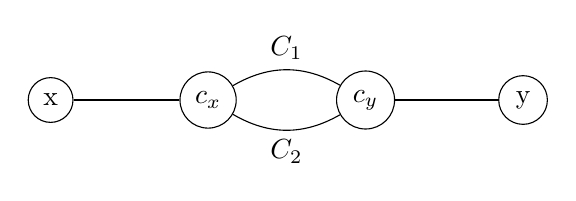
\begin{tikzpicture}
 	% Nodes
 	\node[circle, draw, fill=white] (c_x) at (0,0) {$c_x$};
 	\node[circle, draw, fill=white] (c_y) at (2,0) {$c_y$};
 	\node[circle, draw, fill=white] (x) at (-2,0) {x};
 	\node[circle, draw, fill=white] (y) at (4,0) {y};
 	% Edges
 
 	\draw[bend right] (c_y) to node[midway, above] {$C_1$} (c_x);
 	\draw[bend right] (c_x) to node[midway, below] {$C_2$} (c_y);
 	\draw (x) -- (c_x) node[midway, above] {};
 	\draw (y) -- (c_y) node[midway, above] {};
 \end{tikzpicture}
 

\clearpage



\subsection{Exercício 3: Seja $G$ um grafo conexo, $T_1$,$T_2$ árvores geradoras distintas de $G$, e seja, $e_1$ uma aresta de $T_1$. Prove que existe uma aresta $e_2$ em $T_2$ tal que $T_1 - e_1 + e_2$ é uma árvore geradora de $G$.}

Considere o seguinte grafo formado pela adicao de uma aresta de $T_2$ a $T_1$:

 $$
 T_1' = T_1 + e_2
 $$
 
Dessa forma, $T_1'$ certamente possui um ciclo, porque a adicao de qualquer aresta a $T_1$, que é uma árvore, gera um ciclo.

O ciclo formado em $T_1'$ evidentemente contem a aresta $e_2$ e mais duas arestas distintas que podemos definir como $e_1, e_1' \in E(T_1)$, porque todo ciclo possui pelo menos tres arestas distintas.


A retirada de $e_1$ de $T_1'$ desfaz seu único ciclo e mantem o mesmo numero de componentes, porque ciclos nao possuem arestas de corte. Ou seja, $T_1 - e_1 + e_2$ permanence conexo e nao possui ciclos, além de preservar todos os vértices de $T_1$ e, portanto, de $G$. Assim, $T_1 - e_1 + e_2$ é árvore geradora de $G$ .

Provou-se que existe uma aresta $e_2$ em $T_2$ tal que $T_1 - e_1 + e_2$ é uma árvore geradora de $G$.
\clearpage

 \subsection{Exercício 4: Uma $k$-coloração dos vértices de um grafo é uma atribuição de no máximo $k$ cores distintas aos vértices desse grafo, tal que vértices adjacentes recebem cores distintas. Dizemos que um grafo é equi-bicolorido se tem uma 2-coloração com igual número de vértices de cada cor. Prove que toda árvore equi-bicolorida tem pelo menos uma folha de cada cor.}
 
 Sejam $C_1$ e $C_2$ os conjuntos disjuntos de vértices de cor $1$ e $2$, respectivamente, da árvore equi-bilocorida $T$. Assim:
 
 
 \begin{align*}
  v(T) &= v(C_1) + v(C_2) \\
  v(C_1) &= v(C_2)
 \end{align*}
 
Provemos primeiramente que $T$ tem exatamente $v(T)  - 1$ arestas, pois $T$ é  árvore. Utilizemos inducao no número de vértices de $T$.

\subsubsection*{Caso Base}

 Quando $v(T) = 1$, $T$ possui $v(T) - 1 = 0$  ciclo. Ou seja, quando $T$ é uma árvore de apenas $1$ vértice, $T$ tem um número de arestas igual a um menos o seu número de vértices.
 
 \subsubsection*{Hipótese de Inducao}
 
 Suponhamos que vale a afirmacao para qualquer árvore com estritamente menos do que $k$ vértices, $k > 1$.
 
 Seja $f$ uma folha de uma árvore $T$ com $k$ vértices. Seja $T'$ o grafo:
 
 $$
 T' = T \setminus \{f\}
 $$
 
 A remocao de $f$ de $T$ nao resultou num $T'$ desconexo, pois uma folha nao possui nenhuma aresta de corte adjascente a si.
 
 Ademais, $T'$ nao tem nenhum ciclo, pois é impossível criar ciclos apenas retirando-se vértices de uma árvore. Ou seja, $T'$ é conexo e acíclico tal qual $T$, sendo, portanto, árvore. Além disso, $T'$ tem $k - 1$ vértices e, por hipótese, tem $(k - 1) - 1 = k - 2$ arestas.
 
 Como $f$ retirado de $T$ é folha, ele possui apenas uma aresta adjascente em $T$. Portanto, a adicao de $f$ em $T'$ para formar $T$ de volta acrescenta uma única aresta. Portanto, $e(T) = e(T') + 1 = k - 2 + 1 = k - 1$. Portanto, $T$ é uma árvore com $k$ vértices e $k - 1$ arestas.
 
 
Suponhamos, por absurdo, que $C_1$ nao possui nenhuma folha. Assim, o grau de qualquer vértice de $C_1$ é de pelo menos $2$ e, portanto, $G$ tem pelo menos $2v(C_1)$, já que $C_1$ nao possui nenhum par de vértices vizinhos.

$$
e(G) \geq 2 || C_1 || = 2v(C_1)
$$

$G$ é árvore e, como demonstrado, tem exatamente $v(G) - 1$ arestas. 

 \begin{align*}
	e(G) &= v(G) - 1  \\
	        &= v(C_1) + v(C_2) - 1 \\
	        &\geq 2v(C_1) \\
	        &\implies v(C_2) \geq v(C_1) + 1 \\
	        &\implies v(C_2) >  v(C_1)  
\end{align*}

O que é uma contradicao, pois $v(C_1) = v(C_2)$, já que $G$ é bicolorida. Portanto, a suposicao inicial de que $C_1$ nao possui nenhuma folha é falsa e ambos conjuntos disjuntos $C_1$ e $C_2$ possuem pelo menos uma folha cada um.

 \clearpage
 
 \subsection{Exercício 7: Prove que um grafo conexo $G$ é euleriano se, e só se, $G$ contém ciclos $C_1, C_2, \ldots, C_k$ dois a dois disjuntos nas arestas tais que $E(G) = E(C_1) \cup E(C_2) \cup \cdots \cup E(C_k)$.}

\subsubsection{Prova  de que dado um grafo conexo e euleriano $G$ implica que existem ciclos $C_1, \ldots, C_k$ disjuntos nas arestas tais que a união de todos eles resulta em $E(G)$ — as arestas de $G$.}

Seja $N = V(G)$ o número total de vértices distintos em um grafo conexo euleriano $G$ minimal no número de arestas. Como uma condicao necessaria e suficiente para $G$ ser euleriano é que todos os seus vértices tenham grau par e $G$ tem o menor número de arestas possível por suposicao, $d_G(u) = 2$ para todo vértice $u$ em $G$. 

\subsubsection*{Caso Base}
$N = 3$ \\
Quando $G$ possui apenas 3 vértices, é euleriano e conexo, pode-se definir o ciclo  $C_1 = E(G)$ e $C_2 = \emptyset$ . Evidentemente, $E(C_1) \cap E(C_2) = \emptyset$ e $E(C_1) \cup E(C_2) = E(C_1) \cup \emptyset = E(C_1) = E(G)$.

\subsubsection*{Hipótese de Indução}
Seja $G$ tal que $N = V(G) =  a >  3$. Seja $G$ um grafo minimal em arestas, ou seja, é um grafo que tem o número mínimo de arestas para manter-se conexo e euleriano.  Suponhamos que a afirmação a ser provada é verdadeira para $G$, ou seja, existem $k$ ciclos $C_1, \ldots, C_k$ em $G$ disjuntos nas arestas tais que:

$$E(G) = E(C_1) \cup E(C_2) \cup \cdots \cup E(C_k)$$.


Seja $u \in V(C_i)$ um vértice de $G$. Seja o subgrafo $G' \subset G$, tal que $V(G) = V(G') \cup \{u\}$. Ou seja, $G'$ é o grafo resultante da retirada do vértice $u$ de $G$ e a adicao de uma aresta descrita a seguir. Assim, $V(G') = V(G) - 1 = a - 1$.

Sabemos que $u$ está contido em pelo menos um ciclo $C_i$ de $G$. Isto é:

$$C_i = (x_1, \ldots, x_{u-1}, u, x_{u+1}, \ldots, x_1)$$


Por hipótese, $d(x_{u-1}) = d(x_{u-1}) = 2$. Ou seja, esses vértices sao vizinhos a $u$ em $G$ e a apenas outro vértice também pertencente a $C_i$, sendo eles  $x_{u-2}$ e  $x_{u+2}$. Assim, a minimalidade no número de arestas de $G$ permite afirmar que  $(x_{u-1}, x_{u+1}) \notin E(G)$. Podemos, entao, definir $G'$ como:

\begin{align}
	G' = 
	\begin{cases} 
		E(G') = E(G) \cup \{(x_{u-1}, x_{u+1})\} , \\
		V(G') = V(G) \setminus \{u\}, \text{   } u \in V(G)  \\
	\end{cases}
\end{align},

Na formacao de $G'$, os graus de $x_{u-1}$ e $x_{u+1}$ diminuem em $1$ unidade e $G$ e ficam iguais a $1$, mas logo voltam a ser iguais a $2$ com a adicao da aresta $(x_{u-1}, x_{u+1})$  a $E(G')$. O ciclo $C_i$ deixa de existir, porque $u$ é retirado dele, mas surge o ciclo $C'_i \subset G'$:

$$C'_i = (x_1, \ldots, x_{u-1}, x_{u+1}, \ldots, x_1)$$

Como $d(u) = 2$ e $u$ é adjascente a dois vértices distintos em $C_i$, é possível afirmar $\forall j \neq i, u \notin V(C_j) $. Ou seja, é possível afirmar que o vértice $u$ retirado de $G$ para formar $G'$ é pertencente a apenas um dos ciclos $C_i$ dos ciclos disjuntos nas arestas de $G$.
Assim, é possível afirmar:

$$
E(G') =    E(C'_i) \cup \bigcup_{j \neq i} C_j 
$$
$$
C_j \in \{C_1, \ldots, C_k\}
$$

Ou seja, os ciclos $C_j$ disjuntos nas arestas cuja uniao resulta em $G$ contem todas as arestas de $G'$ com excecao da aresta $(x_{u-1}, x_{u+1})$ contida em $C'_i$.

Além disso, $C'_i \cap C_j = \emptyset$, pois $C'_i$ contém arestas de $C_i$ e uma aresta $(x_{u-1}, x_{u+1})$ nao pertencente a $G$ e nao pertencente a nenhum de seus ciclos por consequencia.

Os graus dos vértices de $G'$ sao todos pares, portanto $G'$ é euleriano. $G'$ é conexo, pois a aresta $(x_{u-1}, x_{u+1})$ substitui qualquer trilha que passe por $ x_{u-1}, u ,  x_{u+1}$ em $G$.

Conclui-se que $G'$, é um grafo conexo e euleriano tal que $V(G') = a - 1$ e para o qual foi possível encontrar um conjunto de ciclos disjuntos nas arestas cuja uniao das arestas resulta em todas as arestas de $G'$. Assim, fica provado por inducao a validade da afirmacao para qualquer grafo conexo e euleriano $G$.

 
  \subsubsection{Prova de que se um grafo  $G$ é tal que existem ciclos $C_1, \ldots, C_k$ disjuntos nas arestas cuja união resulta em $E(G)$ — as arestas de $G$, entao $G$ é conexo e euleriano.}
 
Seja $k_{max}$ o tamanho do maior conjunto de ciclos de $G$ disjuntos nas arestas cuja uniao resulta em $G$. 
 
 \subsubsection*{Caso Base}
 $k_{max} = 0$ \\
O grafo representado por um único vértice é tal que pode-se definir um ciclo vazio que contem todas as arestas do grafo, que é outro conjunto vazio. Evidentente, esse ciclo é disjunto nas arestas com outros ciclos do grafo, já que e;e nao tem aresta nenhuma. Esse grafo é conexo, pois possui apenas um vértice, e é euleriano, pois o grau de seu único vértice é par igual a $0$.
 
 \subsubsection*{Hipótese de Inducao}
 Suponhamos que existe um grafo $G$ para o qual vale a afirmacao. Selecionemos o maior $k_{max} = k_{max_G}$ tal que a afirmacao permaneca válida, i.e., selecionemos o maior conjunto de ciclos de $G$ disjuntos nas arestas cuja uniao resulta em $G$. $k_{max_G}$ sempre existe, porque se o conjunto de ciclos é único entao seu tamanho é o máximo e se nao for, há algum  conjunto de ciclos maior ou igual a todos os outros. 
 
 Seja $E'= E(G) \setminus E(C_i), i \in [k]$, i.e., $G'$ é o grafo resultante da retirada das arestas de $C_i$ de $G$. Por hipótese, $E(C_i) \cap E(C_j) = \emptyset, i\neq j$ Podemos afirmar que as arestas dos ciclos $C_j \neq C_i$ também pertencem as arestas de $G'$ e permanecem pertencentes a ciclos disjuntos dois a dois. Ou seja:
 
 $$
 E(G') = E(C_1) \cup \ldots \cup E(C_i) \cup E(C_{i+1}) \cup \ldots E(C_k)
 $$
 $$
 E(C_i) \cap E(C_j) = \emptyset, i\neq j
 $$
 
 Resta mostrar que $G'$ é conexo e euleriano.
 
 $G'$ contem as mesmas arestas de $G$ menos aquelas de $C_i$. A retirada das arestas de $C_i$ para formar $G'$ nao altera em nada os caminhos entre os vértices dos ciclos $C_j \neq C_i$, pois eles sao disjuntos nas arestas por hipótese. Assim, tais vértices permanecem conectados e $G'$ é conexo.
 
 Agora, resta mostrar que $G'$ é euleriano.
 
 Seja $v \in V(C_i)$ e $v \in V(C_j), C_j \neq C_i$, i.e., $v$ é um vértice de $C_i$ que também está em algum outro ciclo $C_j$.
 
 Sabe-se que o grau de $v$ em $G$ é par, pois $G$ é euleriano por hipótese. O grau de $v$ em $C_i$ também é par, pois $C_i$ é um ciclo. Assim, podemos afirmar:
 
 $$
 d_{G'}(v) = d_G(v) - d_{C_i}(v)
 $$
 
 O grau de $v$ em $G'$ é a subtracao de dois números pares, entao $ d_{G'}(v)$ é par também para qualquer $v$.
 
 Como os vértices $v$ sao os únicos remanescentes em $G'$ cujas adjascencias foram afetadas pela retirada de $C_i$, pode-se concluir que os outros mantem seu grau par. Ou seja, $G'$ possui apenas vértices de grau par e é portanto, euleriano. Mostrou-se que a afirmacao também vale para $G'$, um grafo tal que:
 
 $$k_{max_{G'}} = k_{max_G} - 1$$ 
 
 
 \clearpage
 
 

 
 
 



\end{document}
